\section{Assignment 16.9}
\textbf{Assignment Description}
\begin{figure}[H]
	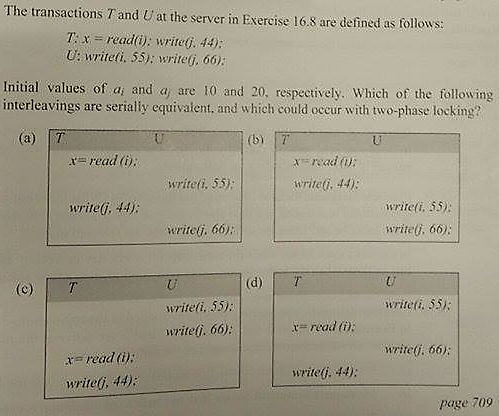
\includegraphics[width = \linewidth]{assignment169}
\end{figure}
Both a), b), c), and d) are serially equivalent. a) is serially equivalent to T before U, b) is serially equivalent to T before U, c) is serially equivalent to U before T, d) is serially equivalent to U before T.\\\\
The 2-phase-locking protocol states that a transaction must handle its locks in two distinct, consecutive phases during the transaction's execution:
\begin{enumerate}
	\item \textbf{Expanding phase}' (aka Growing phase): locks are acquired and no locks are released (the number of locks can only increase).
	\item \textbf{Shrinking phase}: locks are released and no locks are acquired.
\end{enumerate}
You can do this in all the interleavings, and so they could all happen with 2PL. b) and c) are the most obvious choices because T comes before U and U comes before T, which clearly makes it possible to acquire locks and release them. But also a) and )d could be done with 2PL. For a) you could just lock both \textit{i} and \textit{j} for T in the beginning and then release them one at a time, then lock them one at a time for U and release all of them in the end.\\
For d) you could use the same strategy just starting with the locks for U and then for T.